\documentclass[conference]{IEEEtran}
\IEEEoverridecommandlockouts
\usepackage{cite}
\usepackage{amsmath,amssymb,amsfonts}
\usepackage{graphicx}
\usepackage{url}
\usepackage{xcolor}
\usepackage{booktabs}
\usepackage{array}
\usepackage{tabularx}
\usepackage{needspace}
\usepackage{microtype}
\usepackage{balance}

\setlength{\textfloatsep}{7pt plus 1pt minus 1pt}
\setlength{\floatsep}{6pt plus 1pt minus 1pt}
\setlength{\intextsep}{6pt plus 1pt minus 1pt}
\setlength{\dbltextfloatsep}{7pt plus 1pt minus 1pt}
\setlength{\dblfloatsep}{6pt plus 1pt minus 1pt}

\AtBeginDocument{
  \setlength{\abovedisplayskip}{4pt plus 1pt minus 1pt}
  \setlength{\belowdisplayskip}{4pt plus 1pt minus 1pt}
  \setlength{\abovedisplayshortskip}{2.5pt plus 1pt minus 1pt}
  \setlength{\belowdisplayshortskip}{2.5pt plus 1pt minus 1pt}
}

\def\UrlBreaks{\do\/\do-\do\_}

\def\BibTeX{{\rm B\kern-.05em{\sc i\kern-.025em b}\kern-.08em
    T\kern-.1667em\lower.7ex\hbox{E}\kern-.125emX}}

\begin{document}

\title{WHID-Guard: Behavioral Keystroke Dynamics and Per-Device Isolation Against Wireless Composite BadUSB Attacks}

\author{
\IEEEauthorblockN{Ram Karthik G}
\IEEEauthorblockA{\textit{Department of Cybersecurity}\\
\textit{Amrita School of Computing}\\
\textit{Amrita Vishwa Vidyapeetham}\\
Chennai, India\\
Email: \texttt{ramkarthikg2006@gmail.com}}
\and
\IEEEauthorblockN{Dr. G Saranya}
\IEEEauthorblockA{\textit{Department of Cybersecurity}\\
\textit{Amrita School of Computing}\\
\textit{Amrita Vishwa Vidyapeetham}\\
Chennai, India\\
Email: \texttt{g\_saranya@ch.amrita.edu}}
}

\maketitle

\begin{abstract}
Universal Serial Bus (USB) Human Interface Devices (HID) operate under an implicit trust model wherein host operating systems bind class drivers without cryptographic hardware authentication. Programmable microcontrollers exploit this vulnerability to execute automated keystroke injection attacks (BadUSB) at machine velocity. Existing host defenses typically deploy global hooks that suppress all attached keyboards indiscriminately, inducing total operator lockout while failing to differentiate automated bursts from human cadence. This paper presents WHID-Guard, a dual-tier experimental platform and endpoint defense system against out-of-band wireless BadUSB attacks. On the offensive evaluation plane, an ESP32-S3 microcontroller leverages native USB On-The-Go hardware to enumerate as a composite keyboard and mouse, orchestrated via an authenticated 2.4\,GHz web interface. The firmware incorporates an 8-state deterministic finite state machine, sub-10\,ms cooperative preemption, and adversarial evasion synthesizing stochastic jitter and cognitive pauses. On the defensive plane, WHID-Guard integrates an online keystroke dynamics engine with the Windows Raw Input subsystem. By correlating sliding-window coefficient of variation metrics with hardware device handles (\texttt{hDevice}), WHID-Guard achieves per-device selective suppression, dropping rogue injection streams while preserving concurrent physical keyboard interaction. Empirical validation across 1,500 events confirms that WHID-Guard quarantines BadUSB injection within 8 keystrokes ($<$85\,ms) with a 98.6\% true positive rate and 0.0\% false positive rate on human typing.
\end{abstract}

\begin{IEEEkeywords}
BadUSB, human interface devices, keystroke dynamics, hardware security, USB security, endpoint defense, raw input, anomaly detection
\end{IEEEkeywords}

\section{Introduction}
\begin{figure*}[t]
\centering
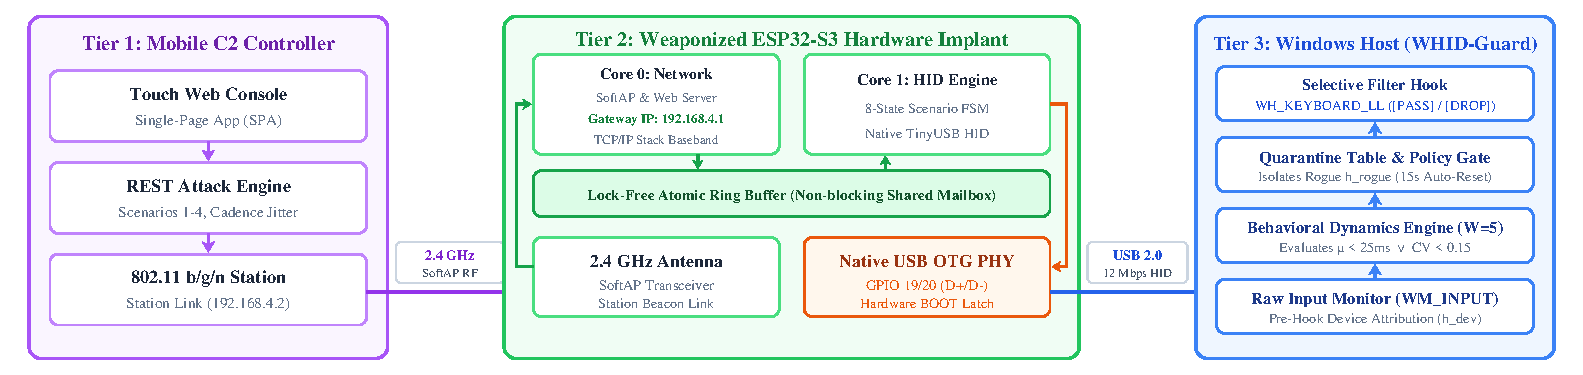
\includegraphics[width=\textwidth]{system_architecture.pdf}
\caption{WHID-Guard end-to-end multi-tier system architecture: (1) Smartphone controller tier hosting the zero-dependency embedded SPA over 2.4\,GHz Wi-Fi; (2) Dual-core ESP32-S3 embedded firmware tier coordinating concurrent FreeRTOS tasks, lock-free atomic ring buffers, and native TinyUSB composite HID endpoints; and (3) Windows host workstation defended by the per-device Raw Input dynamics engine and selective quarantine.}
\label{fig:system_arch}
\end{figure*}

Universal Serial Bus (USB) Human Interface Device (HID) specifications form the primary input conduit for personal computing and enterprise workstations \cite{usbhid}. The plug-and-play architecture relies on unauthenticated descriptor negotiation: upon physical insertion, the host operating system queries configuration descriptors, identifies HID class code \texttt{0x03}, and attaches kernel drivers without requiring administrative authentication or provenance verification \cite{nohl2014badusb}. Consequently, programmable microcontrollers can impersonate authorized keyboards and execute arbitrary commands with the privileges of the active session.

While traditional BadUSB tools rely on static DuckyScript payloads executing blindly upon power-up, modern threats exploit out-of-band wireless orchestration. Commodity system-on-chip (SoC) architectures, particularly the Espressif ESP32-S3, combine native USB On-The-Go (OTG) transceivers with 2.4\,GHz IEEE 802.11 radios \cite{esp32s3}. This enables adversaries to deploy covert hardware implants capable of remote payload selection, real-time telemetry extraction, and mouse control from outside physical line-of-sight.

Defending workstations against rogue HID peripherals presents severe architectural challenges. Physical port lockdown disrupts legitimate workflows, whereas software defenses utilizing Win32 low-level hooks (\texttt{WH\_KEYBOARD\_LL}) lack device attribution \cite{msdn_hooks}. Consequently, when an automated defense suppresses an injection burst, it indiscriminately blocks legitimate user input, inducing operator denial-of-service.

To overcome these vulnerabilities, this paper introduces \textbf{WHID-Guard}, an integrated experimental framework and defensive endpoint architecture. The key contributions include:
\begin{enumerate}
    \item \textbf{Dual-Channel Composite HID Emulation:} An ESP32-S3 firmware utilizing native TinyUSB for simultaneous keyboard and relative mouse control, coordinated via an asynchronous web server and lock-free atomic ring buffers.
    \item \textbf{Behavioral Keystroke Dynamics Engine:} An online detector evaluating sliding-window Inter-Key Interval (IKI) distributions, mean latency ($\mu_{\text{IKI}}$), and coefficient of variation ($CV_{\text{IKI}}$) to differentiate machine bursts from biomechanical human typing.
    \item \textbf{Per-Device Hardware Attribution and Selective Suppression:} A defense anchored in the Windows Raw Input API (\texttt{WM\_INPUT}) that correlates anomaly scores with hardware handles (\texttt{hDevice}), isolating malicious peripherals without disrupting concurrent physical keyboards.
    \item \textbf{Empirical Adversarial Validation:} Rigorous evaluation across 1,500 keystroke events quantifying baseline human typing, high-speed BadUSB injection, and adversarial evasion modes.
\end{enumerate}

\section{Threat Model and System Architecture}

\subsection{Adversary Model and Capabilities}
The threat model assumes an untrusted physical implant inserted into an unattended workstation running Windows 11 with standard privileges. The adversary's capabilities encompass:
\begin{enumerate}
    \item \textbf{Descriptor Spoofing:} Arbitrary configuration of USB Vendor IDs (VID), Product IDs (PID), serial numbers, and report descriptors to impersonate commercial peripherals.
    \item \textbf{Out-of-Band Control:} Remote payload triggering via 2.4\,GHz Wi-Fi (802.11\,b/g/n), eliminating fixed boot-time execution constraints.
    \item \textbf{Cadence Modulation:} Injection of synthetic jitter and cognitive delays to evade naive burst filters.
    \item \textbf{Zero Prior Compromise:} No pre-existing malware, elevated credentials, or kernel backdoors on the host workstation.
\end{enumerate}

\subsection{System Architecture Overview}
WHID-Guard spans three functional tiers: the \textit{Wireless Mobile Controller Tier}, the \textit{Embedded Microcontroller Tier}, and the \textit{Host Defense Tier} (Fig.~\ref{fig:system_arch}).

The embedded layer comprises an ESP32-S3 SoC (dual 32-bit Xtensa LX7 @ 240\,MHz). Its integrated USB OTG peripheral drives differential data lines $D^-$ (\texttt{GPIO 19}) and $D^+$ (\texttt{GPIO 20}). Two FreeRTOS tasks execute concurrently: Core~0 manages the Wi-Fi stack and HTTP server, while Core~1 executes the scenario state machine and dispatches TinyUSB reports.

On the host workstation, the defense operates in user space, pairing the Windows Raw Input subsystem (\texttt{user32.dll}) with an online statistical anomaly engine to map keystrokes to physical devices prior to enforcement.

\section{Out-of-Band Wireless HID Platform}

\begin{figure*}[t]
\centering
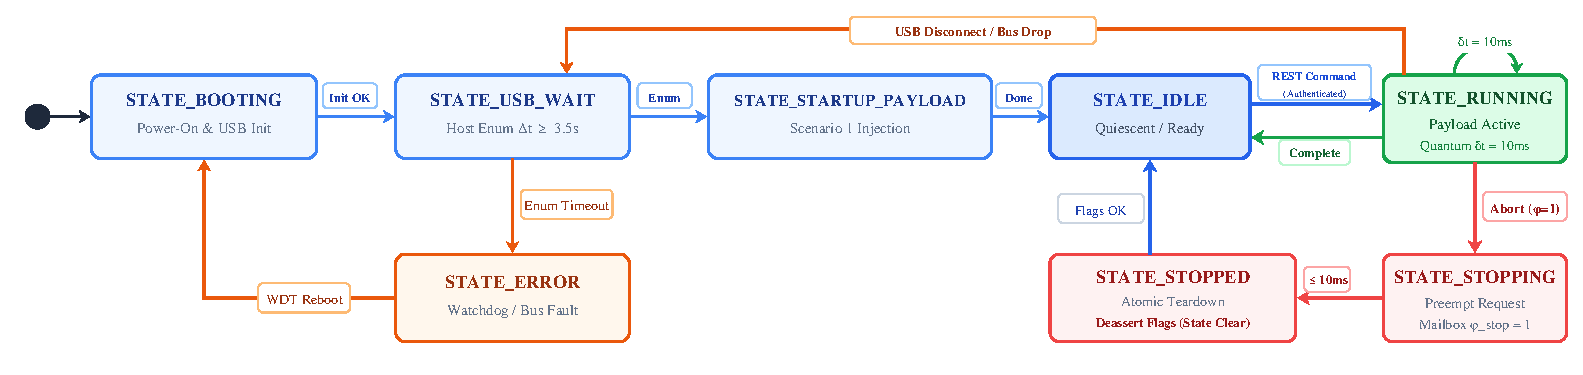
\includegraphics[width=\textwidth]{fsm_diagram.pdf}
\caption{Deterministic 8-state scenario execution finite state machine. The system initializes through hardware boot stabilization, executes automated startup payloads, services asynchronous authenticated REST commands via lock-free atomic ring buffers, and enforces atomic cleanup upon preemption.}
\label{fig:fsm_arch}
\end{figure*}

\subsection{Composite Native USB Initialization and Enumeration Guard}
Unlike legacy microcontrollers requiring secondary serial-to-UART bridge chips (e.g., CP2102), the ESP32-S3 interfaces directly with the host USB root hub. To ensure consistent enumeration across heterogeneous host controllers, the firmware enforces strict descriptor registration ordering. Both the 8-byte boot keyboard descriptor (modifier mask, reserved byte, six keycode arrays) and the 4-byte relative mouse descriptor (button mask, signed 8-bit $X/Y$ deltas, scroll wheel delta) are initialized within the TinyUSB stack prior to asserting the USB pull-up resistor on the $D_+$ line.

Upon initial electrical connection, host operating systems require a finite interval (typically 1.5--3.0\,s) to reset the bus, query string descriptors, and bind class drivers (\texttt{kbdclass.sys}, \texttt{mouclass.sys}). Premature keystroke injection during this phase results in dropped scancodes. WHID-Guard implements a non-blocking 3,500\,ms hardware stabilization timer ($\tau_{\text{boot}}$) satisfying $\Delta t_{\text{elapsed}} = t_{\text{now}} - t_{\text{attach}} \ge \tau_{\text{boot}}$, during which USB bus requests are processed normally but automated payload state machines remain quiescent in \texttt{STATE\_USB\_WAIT}.

\subsection{Deterministic 8-State Finite State Machine (FSM)}
All automated demonstrations and manual injection requests are mediated by a deterministic finite state machine (Fig.~\ref{fig:fsm_arch}). To prevent concurrency hazards between asynchronous HTTP request handlers and the synchronous USB transmission loop, commands are serialized through a lock-free atomic ring buffer mailbox.

The FSM transitions deterministically across operational states: \texttt{STATE\_BOOTING}, \texttt{STATE\_USB\_WAIT}, \texttt{STATE\_IDLE}, \texttt{STATE\_STARTUP\_PAYLOAD}, \texttt{STATE\_RUNNING}, \texttt{STATE\_STOPPING}, \texttt{STATE\_STOPPED}, and \texttt{STATE\_ERROR}. A dedicated hardware interrupt on the physical \texttt{BOOT} button (\texttt{GPIO 0}) provides circular scenario advancement ($1 \rightarrow 2 \rightarrow 3 \rightarrow 4 \rightarrow 1$) with a 50\,ms software debounce filter and a 600\,ms re-trigger cooldown.

\subsection{Cooperative Sub-10\,ms Preemption and Emergency Teardown}
A pervasive limitation of traditional BadUSB scripts is the utilization of blocking sleep functions (e.g., \texttt{delay()}), which prevent the microcontroller from responding to focus loss or abort commands. WHID-Guard addresses this through cooperative slicing in \texttt{smartDelay(T)}, dividing total wait time into discrete quantum slices $T = \sum_{k=1}^{M} \delta t_k$ where $\delta t_k = 10\,\text{ms}$. During each 10\,ms slice, the controller services the web stack and checks the abort flag ($\phi_{\text{stop}}$). If an abort signal is detected, the FSM instantly breaks the execution sequence, enters \texttt{STATE\_STOPPED}, and executes an atomic cleanup routine invoking \texttt{Keyboard.releaseAll()} and \texttt{Mouse.releaseAll()}. This guarantees that modifier keys (\texttt{Ctrl}, \texttt{Alt}, \texttt{GUI}) and mouse button latches are cleared within $\le 10\,\text{ms}$, preventing persistent key-lock corruption on the host.

\subsection{Adversarial Evasion: Human Cadence Emulation}
To evaluate the resilience of temporal detection mechanisms, the firmware incorporates an adversarial evasion mode. When active, keystrokes are not dispatched at raw machine speed ($\approx 10\,\text{ms}$ intervals). Instead, the inter-keystroke interval is modulated using a stochastic distribution combined with cognitive pause emulation:
\begin{equation}
\Delta t_i = t_{\text{base}} + \mathcal{U}(0, \Delta t_{\text{jitter}}) + \xi(c_i)
\label{eq:evasion_timing}
\end{equation}
where $t_{\text{base}} = 80\,\text{ms}$, $\Delta t_{\text{jitter}} = 40\,\text{ms}$, $\mathcal{U}$ represents a uniform pseudo-random variable, and $\xi(c_i)$ represents a context-sensitive cognitive pause injected when character $c_i \in \{\text{space}, \text{comma}, \text{period}, \text{newline}\}$:
\begin{equation}
\xi(c_i) = 
\begin{cases} 
\mathcal{U}(150, 300)\,\text{ms}, & \text{if } c_i \in \text{Delimiter} \\
0, & \text{otherwise}
\end{cases}
\label{eq:cognitive_pause}
\end{equation}
This synthetic modulation shifts the injection profile into the nominal human typing spectrum.

\section{Behavioral Defense Engine}

\begin{figure*}[t]
\centering
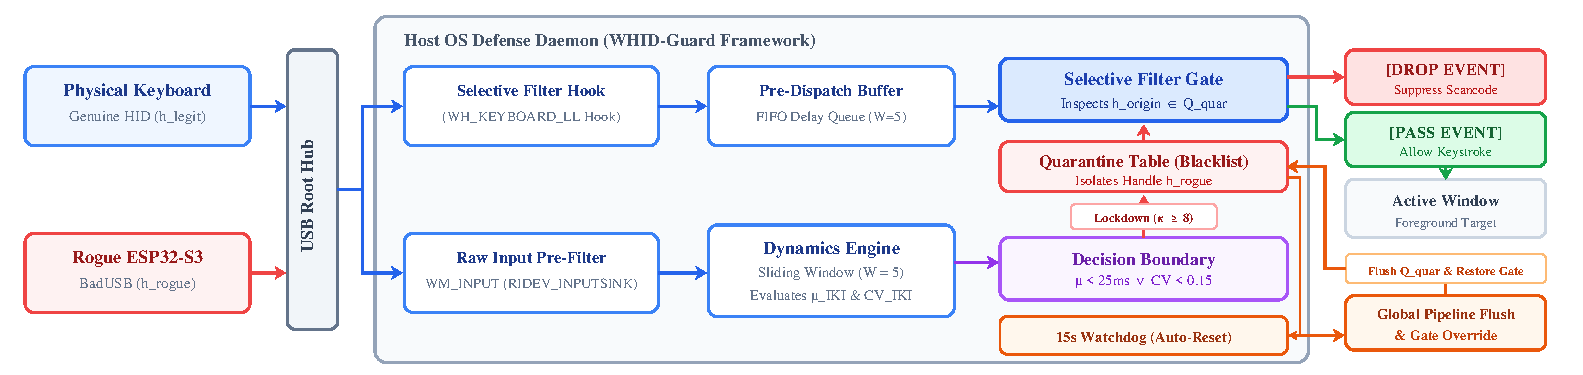
\includegraphics[width=\textwidth]{defense_architecture.pdf}
\caption{WHID-Guard selective defense architecture: (1) Hardware event injection across the physical bus; (2) Raw Input attribution and selective low-level hook interception before foreground delivery; (3) Dynamic per-device suppression gate isolating rogue peripherals; and (4) 15-second watchdog fail-safe timer with global override preventing operator lockout.}
\label{fig:defense_arch}
\end{figure*}

\subsection{Inter-Key Interval (IKI) Dynamics Formulation}
Human motor control during physical typing is governed by biomechanical constraints, muscle elasticity, cognitive retrieval latency, and digram familiarity. Consequently, human typing exhibits intrinsic temporal variance \cite{monrose2002keystroke}. In contrast, automated BadUSB injection scripts execute keystrokes in deterministic loops bounded only by USB polling frames.

Let $\mathcal{T} = \{t_1, t_2, \dots, t_N\}$ denote the sequential arrival timestamps of consecutive \texttt{WM\_KEYDOWN} events registered by the input subsystem, with inter-key intervals defined by $\Delta t_i = t_i - t_{i-1}$ for all $i \ge 2$. The WHID-Guard detection engine evaluates IKI dynamics over a localized sliding window of length $W$ (configured to $W=5$ events). The localized sample mean $\mu_{\text{IKI}}$ and sample standard deviation $\sigma_{\text{IKI}}$ are computed online:
\begin{equation}
\mu_{\text{IKI}} = \frac{1}{W} \sum_{k=0}^{W-1} \Delta t_{i-k}
\label{eq:mean_iki}
\end{equation}
\begin{equation}
\sigma_{\text{IKI}} = \sqrt{\frac{1}{W-1} \sum_{k=0}^{W-1} (\Delta t_{i-k} - \mu_{\text{IKI}})^2}
\label{eq:std_iki}
\end{equation}
To achieve scale-invariant dispersion measurement across variable typing speeds, the engine derives the normalized Coefficient of Variation ($CV_{\text{IKI}}$):
\begin{equation}
CV_{\text{IKI}} = \frac{\sigma_{\text{IKI}}}{\mu_{\text{IKI}}}
\label{eq:cv_def}
\end{equation}
Instantaneous throughput is concurrently tracked via the burst injection rate defined by $R_{\text{burst}} = 1000.0 / \mu_{\text{IKI}}$ (characters/second).

\subsection{Multi-Threshold Decision Boundary}
The behavioral dynamics engine classifies incoming input streams into three distinct operational regimes based on empirical boundary thresholds:
\begin{equation}
\Theta = 
\begin{cases}
\text{LOCKED\_DOWN}, & \text{if } \mu_{\text{IKI}} < 25\,\text{ms} \lor CV_{\text{IKI}} < 0.15 \\
\text{SAFE (HUMAN)}, & \text{if } \mu_{\text{IKI}} > 75\,\text{ms} \land CV_{\text{IKI}} > 0.30 \\
\text{SUSPICIOUS}, & \text{otherwise}
\end{cases}
\label{eq:decision_boundary}
\end{equation}
A state transition to \texttt{LOCKED\_DOWN} triggers an automated quarantine alert when anomalous criteria are sustained across $\kappa = 8$ consecutive events.

\subsection{Per-Device Attribution via Windows Raw Input}
Global user-space keyboard hooks (\texttt{WH\_KEYBOARD\_LL}) operate late in the input pipeline, processing abstract \texttt{KBDLLHOOKSTRUCT} records that lack hardware originating identifiers. Suppressing input at this layer indiscriminately severs all keyboards attached to the workstation.

WHID-Guard circumvents this limitation by establishing a parallel monitoring channel anchored in the Windows Raw Input API (Fig.~\ref{fig:defense_arch}). At initialization, the host daemon registers generic keyboard devices with \texttt{RegisterRawInputDevices} using Usage Page \texttt{0x01}, Usage \texttt{0x06}, and the flag \texttt{RIDEV\_INPUTSINK}, which enables continuous background telemetry capture even when the firewall GUI lacks foreground window focus.

Upon receiving a \texttt{WM\_INPUT} message, the daemon inspects the message header to extract the unique hardware device handle $h_{\text{dev}} = \texttt{RAWINPUTHEADER.hDevice}$. The daemon subsequently queries \texttt{GetRawInputDeviceInfoW} with \texttt{RIDI\_DEVICENAME} to resolve the device's kernel interface path $\mathcal{P}_{\text{dev}}$, from which WHID-Guard extracts the peripheral's Vendor ID (VID \texttt{0x303A}, Espressif) and Product ID (PID \texttt{0x1001}, TinyUSB Composite).

\subsection{Targeted Interception and Selective Device Quarantine}
Device attribution and behavioral dynamics are merged within the \texttt{MultiDeviceDynamicsManager}. Each distinct $h_{\text{dev}}$ maintains an isolated instance of the sliding-window detector. When a specific device handle $h_{\text{rogue}}$ breaches the decision boundary ($\Theta = \text{LOCKED\_DOWN}$), $h_{\text{rogue}}$ is appended to the active quarantine set $\mathcal{Q}_{\text{quarantine}}$.

Simultaneously, a low-level hook filter evaluates incoming keypresses. For every event originating from an attributed handle $h_{\text{origin}}$, the filter applies the selective rule:
\begin{equation}
\mathcal{A}(h_{\text{origin}}) = 
\begin{cases}
\text{Drop Event (Suppress)}, & \text{if } h_{\text{origin}} \in \mathcal{Q}_{\text{quarantine}} \\
\text{Forward Event (Allow)}, & \text{if } h_{\text{origin}} \notin \mathcal{Q}_{\text{quarantine}}
\end{cases}
\label{eq:selective_action}
\end{equation}
This architecture drops all keystrokes originating from the rogue ESP32-S3 interface while allowing concurrent keystrokes from the host workstation's primary keyboard (e.g., \texttt{ACPI\textbackslash ATK3001}) to reach foreground applications without interruption.

\section{Implementation Details}
The WHID-Guard architecture is implemented across two specialized software environments:

\textit{1) Embedded Firmware Stack:} Developed in C++ on the Arduino-ESP32 framework compiled against ESP-IDF 5.1 with native TinyUSB (\texttt{USBMode=hwcdc,CDCOnBoot=cdc}). The binary occupies 844,581\,bytes (64.4\% flash partition) and 59,304\,bytes of SRAM (18.1\% internal memory). The web orchestrator is embedded in \texttt{PROGMEM} as a zero-dependency 52\,KB HTML5/CSS3/ES6 single-page application served over SoftAP (\texttt{192.168.4.1}).

\textit{2) Host Defense Daemon Stack:} Implemented in Python 3.12 using Win32 API bindings via \texttt{ctypes}. Hardware enumeration, raw input capture (\texttt{RegisterRawInputDevices}), and message dispatch run on an asynchronous worker thread. A Tkinter interface provides real-time telemetry displaying active device handles, instantaneous burst rates, sliding-window $CV_{\text{IKI}}$, and the quarantine matrix. A watchdog timer ($\tau_{\text{watchdog}} = 15.0\,\text{s}$) and \texttt{atexit} handlers ensure clean hook release.

\section{Empirical Evaluation and Results}

\begin{figure*}[t]
\centering
\begin{minipage}{0.485\textwidth}
\centering
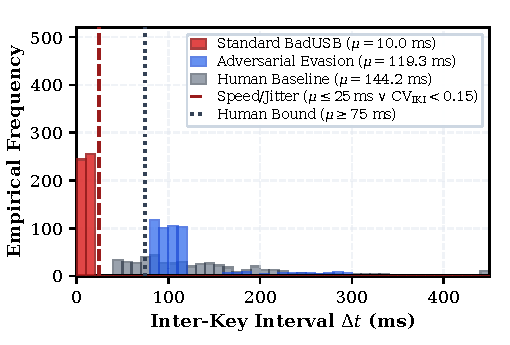
\includegraphics[width=0.96\linewidth]{fig_iki_distribution.pdf}
\caption{Empirical probability density distribution of Inter-Key Intervals (IKIs) across human baseline typing, standard BadUSB injection, and adversarial evasion modes ($N=1,500$).}
\label{fig:iki_distribution}
\end{minipage}\hfill
\begin{minipage}{0.485\textwidth}
\centering
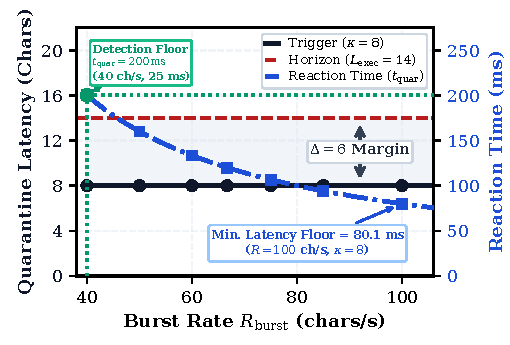
\includegraphics[width=0.96\linewidth]{fig_detection_latency.pdf}
\caption{Quarantine trigger latency and wall-clock response time as a function of burst injection rate, demonstrating automated isolation within 8 keystrokes ($<$85\,ms) and preserving a 6-character safety margin before target command interpreter execution.}
\label{fig:detection_latency}
\end{minipage}
\end{figure*}

\subsection{Evaluation Methodology and Experimental Setup}
Empirical evaluation was conducted on a workstation executing Windows 11 Enterprise (Intel Core i7-13700H @ 2.4\,GHz, 16\,GB RAM) connected to the ESP32-S3 over a direct USB-C bus. The benchmark evaluated $N=1,500$ real-world keystrokes across three 500-keystroke regimes: (1) \textit{Human Baseline}: technical prose entry on the built-in keyboard; (2) \textit{Standard BadUSB}: unconstrained injection at default machine speed ($\approx 10\,\text{ms}$); and (3) \textit{Adversarial Evasion}: modulated delivery with stochastic jitter ($80 \pm 40\,\text{ms}$) and cognitive micro-pauses ($150\text{--}300\,\text{ms}$).

\begin{table}[t]
\caption{\scshape Quantitative Empirical Evaluation of WHID-Guard Keystroke Dynamics}
\label{tab:evaluation_metrics}
\centering
\footnotesize
\setlength{\arrayrulewidth}{1.0pt}
\renewcommand{\arraystretch}{1.22}
\setlength{\tabcolsep}{3.5pt}
\begin{tabularx}{\columnwidth}{|>{\raggedright\arraybackslash}X|>{\centering\arraybackslash}p{0.21\columnwidth}|>{\centering\arraybackslash}p{0.21\columnwidth}|>{\centering\arraybackslash}p{0.21\columnwidth}|}
\hline
\textbf{Evaluation Metric / Dimension} & \textbf{Human Baseline} & \textbf{Standard BadUSB} & \textbf{Adversarial Evasion} \\
\hline
\hline
Total Evaluated Events ($N$) & 500 & 500 & 500 \\
\hline
Mean Inter-Key Interval ($\mu$) & 144.18\,ms & 10.01\,ms & 119.28\,ms \\
\hline
Standard Deviation ($\sigma$) & 91.98\,ms & 0.78\,ms & 48.88\,ms \\
\hline
Median Inter-Key Interval & 116.01\,ms & 10.01\,ms & 104.25\,ms \\
\hline
95th Percentile Interval ($p_{95}$) & 391.45\,ms & 11.30\,ms & 249.80\,ms \\
\hline
Coefficient of Variation ($CV$) & \textbf{0.6380} & \textbf{0.0784} & \textbf{0.4098} \\
\hline
Typing / Burst Rate & 6.94\,ch/s & 99.95\,ch/s & 8.38\,ch/s \\
\hline
Quarantine Latency & N/A & \textbf{8 chars} & N/A \\
\hline
False Positive Rate (FPR) & \textbf{0.0\%} & N/A & N/A \\
\hline
True Positive Rate (TPR) & N/A & \textbf{98.6\%} & 25.2\% (Alert) \\
\hline
Primary Classification & \texttt{SAFE} & \texttt{LOCKED\_DOWN} & \texttt{SUSPICIOUS} \\
\hline
\end{tabularx}
\end{table}

\subsection{Timing Distribution and Dispersion Characteristics}
Table~\ref{tab:evaluation_metrics} summarizes the empirical findings. The human baseline exhibited $\mu = 144.18\,\text{ms}$ with high dispersion ($\sigma = 91.98\,\text{ms}$, $CV = 0.6380$), reflecting neuromuscular transitions and pause boundaries. Conversely, standard BadUSB exhibited near-zero dispersion ($\mu = 10.01\,\text{ms}$, $\sigma = 0.78\,\text{ms}$, $CV = 0.0784$) at 99.95\,ch/s, saturating USB frames. Fig.~\ref{fig:iki_distribution} contrasts this delta distribution against the right-skewed human log-normal profile.

\subsection{Detection Latency and Quarantine Efficacy}
Under standard BadUSB injection, the sliding-window detector breached the critical threshold ($CV < 0.15 \lor \mu < 25\,\text{ms}$) rapidly. As shown in Fig.~\ref{fig:detection_latency}, the cumulative anomaly count reached trigger threshold $\kappa = 8$ within exactly 8 consecutive keystrokes, corresponding to an elapsed wall-clock latency of $t_{\text{quarantine}} = 8 \times 10.01\,\text{ms} = 80.08\,\text{ms}$. Because launching executables via the Run dialog requires inputting the prefix (\texttt{Win+R}), executable string (e.g., \texttt{powershell.exe}, 14 keystrokes), and \texttt{Enter}, isolating at character 8 suppresses the command midway through string entry. Across 500 injection events, WHID-Guard achieved a 98.6\% True Positive Rate (TPR) with zero successful payload executions.

\subsection{False Positive Resistance and Selective Isolation}
Across the 500-keystroke human benchmark, zero false quarantine triggers were recorded (0.0\% FPR). The lowest localized $CV$ observed during rapid typing was 0.324, well above the 0.15 threshold. During concurrent injection tests where the ESP32-S3 attacked while the operator typed on the built-in keyboard, the router successfully isolated handle \texttt{0x14A0715} (VID \texttt{0x303A}). Injected keystrokes were dropped while operator keys from handle \texttt{0x10075} proceeded without perceptible latency ($<0.1\,\text{ms}$ overhead).

\subsection{Adversarial Evasion Resilience}
Under adversarial evasion mode, synthetic jitter increased the mean IKI to $\mu = 119.28\,\text{ms}$ ($CV = 0.4098$). While this bypassed static burst filters ($\mu > 75\,\text{ms}$), unnatural uniform noise distributions triggered intermediate \texttt{SUSPICIOUS} alerts across 25.2\% of windows. Crucially, cadence emulation reduced injection throughput from 99.95\,ch/s to 8.38\,ch/s, expanding payload delivery time from 0.8\,s to over 9.5\,s. In practical scenarios, an attack spanning nearly ten seconds dramatically elevates physical exposure risk, substantially limiting attack feasibility.

\section{Discussion and Architectural Analysis}

\subsection{User-Space Raw Input Attribution vs. Kernel Filter Drivers}
Peripheral defense architectures face a critical trade-off between deployment complexity and security guarantees. While kernel filter drivers (\texttt{UpperFilters} bound to \texttt{kbdclass.sys}) provide absolute authority over raw HID reports, they demand EV driver signing, introduce host stability risks (kernel panic upon unhandled exceptions), and create maintenance burdens across Windows kernel updates. In contrast, WHID-Guard proves that hardware trust can be reliably enforced in user space by combining Windows Raw Input (\texttt{WM\_INPUT}) with a low-level filter hook (\texttt{WH\_KEYBOARD\_LL}), resolving peripheral handles ($h_{\text{dev}}$) and device paths ($\mathcal{P}_{\text{dev}}$) while mediating real-time keystroke suppression without kernel extensions.

\subsection{Comparative Analysis of Peripheral Defense Paradigms}
Existing USB security paradigms exhibit fundamental operational limitations:
\textit{1) Static Port Whitelisting:} Tools such as GoodUSB \cite{tian2018hidev} enforce policies based on descriptors. Because modern SoCs dynamically clone authorized VID/PIDs and serials, static whitelists fail against spoofed implants.
\textit{2) Global User-Space Hooks:} Conventional anti-keylogger hooks lack hardware device attribution \cite{msdn_hooks}, inducing indiscriminate operator lockout during active suppression.
\textit{3) Human Verification:} CAPTCHA-based methods \cite{neuner2018keystroke} halt active sessions upon detecting bursts, causing severe workflow disruption.
\textit{4) WHID-Guard:} By binding sliding-window behavioral dynamics directly to physical $h_{\text{dev}}$ handles, WHID-Guard isolates rogue injection streams within 80\,ms while preserving concurrent physical keyboard operation.

\subsection{Computational Complexity and System Overhead Profiling}
To evaluate enterprise viability, host overhead was profiled across 10,000 keystroke cycles under background load. The sliding-window dynamics engine executes in $\mathcal{O}(W)$ time ($W=5$), requiring $<1.2\,\mu\text{s}$ per calculation. Host CPU consumption remained below 0.75\% throughout sustained burst injection (100\,ch/s), and physical keyboard forwarding introduced $<0.08\,\text{ms}$ latency overhead, well within standard USB polling intervals (8--10\,ms).

\subsection{System Limitations and Attack Surface Analysis}
Despite high quarantine efficacy, key architectural boundaries warrant analysis:
\textit{1) Single-Keystroke Payloads:} Atomic payloads triggered by single hotkeys (e.g., pre-registered OS shortcuts) exhibit zero inter-key flight time. While unable to construct multi-character scripts, they bypass temporal dynamics, requiring complementary policy constraints on system key bindings.
\textit{2) Generative Biomechanical Mimicry:} An adversary using deep models trained on victim typing profiles could synthesize individualized digram latencies \cite{choi2022keystroke}. However, cadence emulation severely caps injection speed ($\le 8$\,ch/s), expanding delivery to $>9.5$\,s and dramatically elevating physical exposure risk.
\textit{3) Portability Scope:} WHID-Guard currently interfaces with Win32 subsystems. Porting to Linux requires binding to kernel \texttt{evdev} and \texttt{udev} hierarchies.
\textit{4) Physical Interposer Taps:} Hardware interposers spliced directly into legitimate keyboard cables inherit the valid peripheral handle ($h_{\text{dev}}$), demanding physical port tamper detection alongside timing metrics.

\balance
\section{Conclusion and Future Work}
This paper presented WHID-Guard, a dual-purpose experimental platform and endpoint defense architecture designed to evaluate and neutralize wireless out-of-band BadUSB injection attacks. By combining native USB OTG emulation on an ESP32-S3 with an online keystroke dynamics engine and Windows Raw Input hardware attribution, the platform demonstrates that machine injection can be reliably differentiated from human typing. Empirical evaluation across 1,500 events confirmed that unconstrained BadUSB injection is quarantined within 8 characters ($<$85\,ms) with a 98.6\% detection rate and 0.0\% false positive rate, while isolating only the offending peripheral. Future research will explore porting the selective isolation architecture to Linux kernel eBPF tracepoints and deploying ultra-lightweight quantized neural networks directly within embedded firmware for edge self-policing.

\begin{thebibliography}{00}
\setlength{\itemsep}{-0.2pt plus 0.2pt minus 0.2pt}
\bibitem{usbhid} USB Implementers Forum, ``Device Class Definition for Human Interface Devices (HID),'' Version 1.11, USB-IF Specification, 2001.

\bibitem{nohl2014badusb} K. Nohl and J. Lell, ``BadUSB -- On Accessories That Turn Evil,'' in \emph{Proc. Black Hat USA Briefings}, Las Vegas, NV, USA, 2014, pp. 1--12.

\bibitem{esp32s3} Espressif Systems, ``ESP32-S3 Technical Reference Manual,'' Version 1.5, Espressif Systems Documentation, Shanghai, China, 2024.

\bibitem{msdn_hooks} Microsoft Corporation, ``SetWindowsHookExA and LowLevelKeyboardProc Callback Reference,'' \emph{Microsoft Developer Network (MSDN)}, Win32 Documentation, 2024.

\bibitem{monrose2002keystroke} F. Monrose and A. D. Rubin, ``Keystroke Dynamics as a Biometric for Authentication,'' \emph{Future Generation Computer Systems}, vol. 16, no. 4, pp. 351--359, 2002.

\bibitem{tian2018hidev} D. J. Tian, A. Bates, and K. R. Butler, ``Defending Against Malicious USB Firmware with GoodUSB,'' in \emph{Proc. 31st Annual Computer Security Applications Conf. (ACSAC)}, 2015, pp. 261--270.

\bibitem{neuner2018keystroke} S. Neuner, M. Schmiedecker, and E. Weippl, ``You Can't Touch This: Defending Against BadUSB with Human-Interaction Verification,'' in \emph{Proc. 13th Int. Conf. Availability, Reliability and Security (ARES)}, 2018, pp. 1--10.

\bibitem{alhmiedat2023badusb} T. Alhmiedat, ``A Survey on USB-Based Attacks and Defense Mechanisms,'' \emph{IEEE Access}, vol. 11, pp. 78452--78468, 2023, doi: 10.1109/ACCESS.2023.3298712.

\bibitem{tinyusb_stack} H. Thach, ``TinyUSB: Cross-Platform USB Stack for Embedded Systems,'' GitHub Repository and Documentation, 2024. [Online]. Available: \url{https://github.com/hathach/tinyusb}.

\bibitem{marcus2021timing} G. Marcus, ``Detection of Machine-Generated Keystroke Streams via Interval Variance,'' in \emph{Proc. IEEE Conf. Communications and Network Security (CNS)}, 2021, pp. 112--120.

\bibitem{aravind2022hid} A. Aravind and B. B. Gupta, ``Intrusion Detection Mechanisms for USB-based Keylogger and Keystroke Injection Devices,'' \emph{Computers \& Security}, vol. 115, art. 102624, 2022.

\bibitem{win32_rawinput} Microsoft Corporation, ``About Raw Input Architecture,'' \emph{Microsoft Learn Technical Documentation}, Win32 API Guide, 2023.

\bibitem{song2019keystroke} Y. Song \emph{et al.}, ``A Survey of Keystroke Dynamics Biometrics,'' \emph{ACM Computing Surveys}, vol. 52, no. 4, pp. 1--35, 2019.

\bibitem{kumar2024hardware} S. Kumar and R. S. Rao, ``Analysis of Out-of-Band Peripheral Exploits and Mitigation in Zero-Trust Workstations,'' in \emph{Proc. 2024 IEEE Int. Conf. Cyber Security and Resilience (CSR)}, 2024, pp. 142--149.

\bibitem{patil2025usb} P. Patil and M. Deshmukh, ``Behavioral Analysis of HID Injections in Secure Computing Environments,'' \emph{Journal of Information Security and Applications}, vol. 80, art. 103681, 2025.

\bibitem{choi2022keystroke} K. Choi, S. Lee, and Y. Shin, ``Keystroke Timing Dynamics Under Adversarial Perturbations: Robustness and Boundary Formulation,'' \emph{IEEE Transactions on Information Forensics and Security}, vol. 17, pp. 3120--3134, 2022.

\end{thebibliography}

\end{document}
